% Name: Vector addition
% Description: The parallelogram rule for adding two vectors, on a light grid.
% Tags: vectors, parallelogram rule, linear algebra

\usetikzlibrary{arrows.meta}

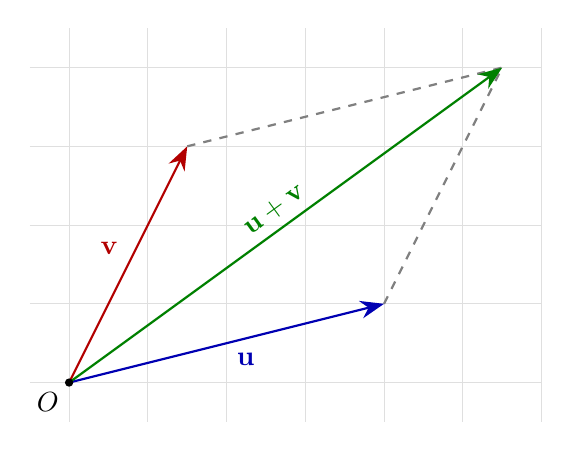
\begin{tikzpicture}[>={Stealth[length=3mm]}, thick]
  \draw[gray!25, thin] (-0.5,-0.5) grid (6,4.5);
  \draw[dashed, gray] (4,1) -- (5.5,4) (1.5,3) -- (5.5,4);
  \draw[->, blue!70!black] (0,0) -- node[below right] {$\mathbf{u}$} (4,1);
  \draw[->, red!70!black] (0,0) -- node[above left] {$\mathbf{v}$} (1.5,3);
  \draw[->, green!50!black] (0,0) -- node[above, sloped] {$\mathbf{u} + \mathbf{v}$} (5.5,4);
  \fill (0,0) circle (1.5pt) node[below left] {$O$};
\end{tikzpicture}
